%=============================================================================
\appendix
%=============================================================================
\chapter{Fusion power and momentum conservation}
\label{appendix:fusion_power}
%=============================================================================

Deuterium-tritium fusion reactions result from inelastic collisions, for which momentum is conserved, not energy. The total kinetic energy release for a single reaction amounts to $\hat E_0 = 17.59$MeV. So as to evaluate the fraction of energy carried out by the neutron, relativistic corrections have to be taken into account. The method is detailed below. \\

Let's admit that it is sufficient to account for relativistic corrections for neutrons only\marginnote{Within the classical framework, one would predict that the neutron carries 4/5 of the total energy, i.e. about $\hat E_n \approx 14.07$MeV. At this energy, it turns out that the velocity of neutrons reaches approximately 17\% of the speed of light ($v_n/c = (2.10^6e\hat E_n/m_n)^{1/2}/c \approx 0.17$). Relativistic corrections cannot be ignored in this case. Conversely, heavier $\alpha$ particles move at about 4\% the speed of light. Relativistic corrections can be neglected for them.}. $\alpha$ particles will be treated within the classical framework.
Momentum conservation then reads:
\begin{equation}
    m_n \gamma_n v_n = m_\alpha v_\alpha
    \label{eq:conserv_momentum}
\end{equation}
with $\gamma_n = (1-v_n^2/c^2)^{-1/2}$ the Lorentz factor for the neutrons. In the limit $v_n/c \ll1$,  $\gamma_n$ can be Taylor expanded, so that Eq.(\ref{eq:conserv_momentum}) can be recast as follows:
\begin{equation}
    u \left( 1+\frac{\epsilon}{2}\; u^2 \right) 
    = 1
    \label{eq:conserv_momentum2}
\end{equation}
with $u \doteq v_n/(\mu v_\alpha)$, $\mu \doteq m_\alpha/m_n$ and $\epsilon \doteq \mu (v_\alpha/c)\ll1$. It is sufficient to look for perturbative solutions of the form: 
$$ u = u_0 + u_1 \;\;\; \textrm{with} \;\; u_1\ll u_0 $$
The leading order yields $u_0=1$. At next order, one readily finds:
$$ u_1 = -\frac{\epsilon^2}{2} \; u_0^3 $$
So that, in the end:
\begin{equation*}
    v_n \simeq \mu v_\alpha \left( 1-\frac{\epsilon^2}{2}\right)
\end{equation*}
where we recall that $\mu=m_\alpha/m_n$.
The kinetic energy of the neutron can then be expressed as a function of the one of the $\alpha$ particle:
\begin{eqnarray*}
    E_n &=& m_nc^2(\gamma_n-1) \approx 
    \frac{1}{2} m_nv_n^2\left[ 1+ \frac{3}{4}\frac{v_n^2}{c^2}\right] \nonumber \\
    &\approx& \mu\; E_\alpha \left( 1-\frac{\epsilon^2}{4}\right)
\end{eqnarray*}

The kinetic energy of the $\alpha$ particle $E_\alpha$ can then be expressed as a function of the total energy $E_0$ ($E_0 =E_\alpha + E_n$). Elementary algebra leads to the following relation:
\begin{equation}
    E_\alpha^2 - \frac{2(1+\mu)}{\mu^2}E_{n0}\, E_\alpha + \frac{2}{\mu^2}\; E_{n0}E_0 = 0
\end{equation}
where $E_{n0} = m_nc^2$ stands for the mass energy of the neutron. We have used the relation $\epsilon^2 = 2\mu\; E_\alpha/E_{n0}$. The only acceptable solution is\marginnote{Notice that, at leading order in $E_0/E_{n0}\ll1$, this solution simply reduces to $E_\alpha \approx E_0/(1+\mu)$.}:
\begin{equation}
    E_\alpha = \frac{1+\mu}{\mu^2}
    \left( 1 - \sqrt{1-\frac{2\mu^2}{(1+\mu)^2}\frac{E_0}{E_{n0}}}\right)\; E_{n0}
\end{equation}
When performing the numerical calculation, it should be warned that $\mu\neq 4$. 
Indeed, the mass of the $\alpha$ particle is slightly less than the sum of its components (actually, this mass difference $\Delta m \approx 0.0187\; m_p$ is the one which leads to the energy release of the D-T fusion reaction $E_0 = \Delta m\;c^2$). The masses can be found in reference \sidecite{Wesson2004}. In particular, $m_n \approx (1+0.001378)\, m_p$ and:
%$$
%    m_n \approx (1+0.001378)m_p \;\;\; ; \;\;\; 
%    m_\alpha = 2(m_n+m_p) \approx (1-0.027404)m_p \approx 3.967\; m_n
%$$
$$
    \mu \doteq \frac{m_\alpha}{m_n} \approx (1-0.027404)\; \frac{m_p}{m_n} \approx 3.967
$$
With these data, one finally obtains $E_0/E_\alpha \approx 4.94$ and $\hat E_\alpha \approx 3.56\,$MeV, which corresponds to the published value.  

%=============================================================================
\chapter{Optimal Temperature for a D-T fusion reactor}
\label{appendix:temperature}
%=============================================================================

As seen on Fig.\ref{fig:reactivity_adv}, the reactivity $\left< \sigma v \right>_{DT}$ of D-T fusion reactions peaks at $T\approx 66.5\,$keV. Yet, this temperature is not the optimal operational one, which rather falls in the range $T\approx 15\,$keV. The reasons are given in this Appendix.


\section{Minimal threshold for the Lawson criterion}

A burning plasma has to satisfy the Lawson criterion, stating that the heating power should overcome the thermal losses. In the case of flat profiles considered in this document, it also reads as follows:
\begin{equation}
 \label{eq:Lawson_general}
 n\tau_E \geq C_{Lawson} 
 \frac{Q}{1+Q/\lambda}
 \frac{\hat T}{\left< \sigma v \right>_{DT}}
\end{equation}
where $C_{Lawson} = 12.10^{-22}/\hat E_{DT}$. It turns out that, within the temperature range $2\,$keV$\leq T \leq 160\,$keV, the reactivity can well be approximated by the following formula proposed by Brunelli (with an error smaller than $7\%$, which drops below $3\%$ in the range $8\leq \hat T \leq 140$ \sidecite{FusionCEA1987}):
\begin{equation}
  \left< \sigma v \right>_{DT} \approx 9.10^{-22}
  \exp\left\{ -0.476 \left| \ln\frac{\hat T}{69} \right|^{2.25}\right\}
  \;\;\;\textrm{m}^3.\textrm{s}^{-1}
\end{equation}
Obviously, the Lawson criterion is all the easier to satisfy since the right hand side of the inequality eq.\ref{eq:Lawson_general} is small. It is is plotted on Fig.\ref{fig:ntauE_Pfus_Tchoice}. It is minimal at $T\approx 26\,$keV, whatever the amplification factor $Q$.

\begin{figure*} 
	\centering
		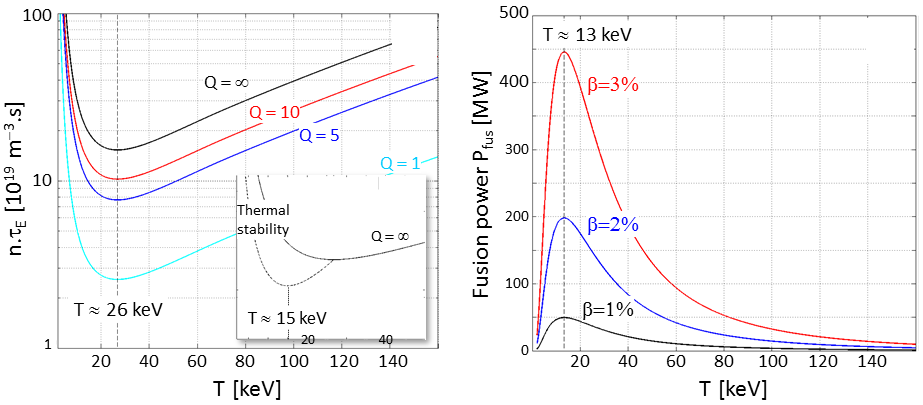
\includegraphics{figures/Fig_ntauE_Pfus_Tchoice_v3.png}
		\caption{Left: threshold for the Lawson criterion. Right: fusion power at prescribed $\beta$.}
		\label{fig:ntauE_Pfus_Tchoice}
\end{figure*}


\section{Thermal stability of the regime}\label{sec:thermal_stability}

Another important criterion has to be accounted for when considering operational regimes, dealing with thermal stability. indeed, the regime is thermally stable provided the total power absorbed by the system is a decreasing function of the temperature (the opposite would lead to a temperature divergence). This constraint translates as follows:
\begin{equation}
  \frac{d (P_{net} - P_{loss})}{dT} \geq 0
  \label{eq:T_stability}
\end{equation}
The accurate computation would require to account for the temperature dependence of ohmic heating $P_\Omega$, of the additional heating power $P_{ext}$ and of the radiative losses $P_{rad}$ involved in the definition of $P_{net}$ (eq.\ref{eq:net_power}), as well as that of the energy confinement time $\tau_E$.

Yet, it is instructive to perform the exercise by neglecting $P_{ext}$ (burning plasma), $P_\Omega$, $P_{rad}$ and the temperature dependence of $\tau_E$. Then, using the expressions of $P_\alpha$ (eq.\ref{eq:P_alpha}) and of $P_{loss}$ (eq.\ref{eq:Ploss}), equation \ref{eq:T_stability} can be recast as follows:
%\begin{equation*}
%\frac{d \left< \sigma v \right>_{DT}}{dT} \leq \frac{12\, \lambda}{E_{DT}} \frac{1}{n \tau_E}
%\end{equation*}
%or alternatively:
\begin{equation}
 %\hat n \tau_E \leq \frac{12.10^{-22}\, \lambda}{E_{DT} \frac{d \left< \sigma v \right>_{DT}}{dT}} 
 \hat n \tau_E \leq \frac{12.10^{-22}\, \lambda}{E_{DT}} 
    \left( \frac{d \left< \sigma v \right>_{DT}}{dT} \right)^{-1} \doteq \left.\hat n \tau_E\right|_{stab}
\label{eq:T_stability_2}
\end{equation}
As evident on Fig.~\ref{fig:ntauE_Pfus_Tchoice} (left, inset), this curve cuts the Lawson curve $\hat n\tau_{E,L}$ at its minimum, which then appears to be a stable solution. In the end, the double product $\hat n\tau_{E}$ satisfying both the Lawson and the thermal stability criteria corresponds, within this simplified approach, to the portion of the plain black curve beyond the minimum at $T\approx 26\,$keV. 
Incidentally, it appears that the minimum stable value is reached at $T\approx 15\,$keV. 


\section{Beta limits}

The fusion power can be expressed in terms of the $\beta$ parameter. It reads:
\begin{equation}
\hat P_{fus} = \frac{C_{fus}}{C_\beta^2} \varepsilon^2 R^3 B^4 
 \frac{\left< \sigma v \right>_{DT}}{\hat T^2}\; \beta 
\end{equation}
If one recognizes that $\beta$, rather than density $n$ and temperature $T$ separately, govern the maximal achievable power in a fusion reactor (due to $\beta$ limits associated to large scale MHD instabilities), one is then led to consider that the optimal temperature is the one that maximizes $\hat P_{fus}$. As shown on Fig.~\ref{fig:ntauE_Pfus_Tchoice}, it peaks at about $T\approx 13\,$keV.


%=============================================================================
\chapter{Constraint on the scaling laws}
\label{appendix:scaling_law_dimensionless}
%=============================================================================

When expressed in engineering variables, the scaling laws for the energy confinement time usually take the following generic form (cf. eq.~\eqref{eq:scaling_law_IPB98(y,2)}):
\begin{equation}
  \label{eq:tauE_SL_generic_a}
  \tau_E \propto \hat M^{\alpha_M} \kappa^{\alpha_\kappa} \varepsilon^{\alpha_\epsilon} \hat n^{\alpha_n} \hat I_p^{\alpha_I} R^{\alpha_R} B^{\alpha_B} \hat P_{net}^{\alpha_P}
\end{equation}
First replacing $\hat I_p$ and $\hat P_{net} = \hat P_{loss}$ by their expressions eqs.~\eqref{eqn:plasma_current} and \eqref{eq:Ploss}, and considering the energy confinement time normalized to the cyclotron frequency $\omega_c = (e/m_p)\, B/\hat M$, eq.~\eqref{eq:tauE_SL_generic_a} yields:
\begin{equation}
\label{eq:tauE_SL_generic_b}
  \omega_c \tau_E \propto 
  \hat M^{\gamma\alpha_M - 1} 
  \kappa^{\gamma(\alpha_\kappa+\alpha_P)} 
  \varepsilon^{\gamma(\alpha_\epsilon+2\alpha_I+2\alpha_P} 
  \hat q^{-\gamma\alpha_I} 
  R^{\gamma(\alpha_R+\alpha_I+3\alpha_P)} 
  B^{1 + \gamma(\alpha_B+\alpha_I)} 
  \hat T^{\gamma\alpha_P}
  \hat n^{\gamma(\alpha_n+\alpha_P)} 
\end{equation}
where the following definition has been introduced:
$$ 
  \gamma \doteq \frac{1}{1+\alpha_P}
$$

Scale invariance properties play a major role in physics: by determining which transforms leave invariant the underlying equations, one can constrain the structure of some key quantities. Especially, as stated in \cite{Connor1977}: ``if the basic equations of plasma behavior [...] are invariant under a certain group of transformations, then any scaling law derived from these equations must be invariant under the same groups of transformations. It turns out that for all the conventional plasma models, this invariance property greatly circumscribes the permissible scaling laws. In other words, even though the necessary non-linear theory may be quite intractable, the mere fact that a scaling law is, in principle, derivable \emph{from certain basic equations} already provides information about that scaling law''.

Now, as we shall see, this property imposes some constraints on the exponents of the scaling law, when expressed in dimensional (or engineering) variables (like Eq.~\ref{eq:tauE_SL_generic_a}). \\

Based on the fact that the system from which the energy confinement scaling law is derived obeys Vlasov' and Maxwell's equations, it can be shown that the associated physics can be described by a reduced set of independent dimensionless parameters, among which the normalized gyro-radius $\rho_*$, the plasma $\beta$ and the collisionality $\nu_*$ \sidecite{Kadomtsev1975, Connor1977}. In that spirit, all dimensional engineering variables entering the scaling of $\tau_E$ (namely $R$, $B$, $\hat n$ and $\hat T_e$) should be able to be recast as functions of $\rho_*$, $\beta$ and $\nu_*$ only when expressed in terms of the dimensionless quantity $\omega_c \tau_E$ (cf. eqs.(14-16) of ref.\cite{ITERphysics_chap2}):
\begin{eqnarray}
  \rho_*  &\doteq& \left( \frac{2.10^3 m_p}{e} \right)^{1/2}\; \frac{(\hat M \hat T_i)^{1/2}}{\varepsilon R B} \\
  \beta   &\doteq& 2.10^{22}e\mu_0\; \frac{\hat n(\hat T_e+\hat T_i)}{B^2} \\
  \nu_*   &\doteq& \nu_{ii}\; \frac{qR \varepsilon^{-3/2}}{(10^3e\, \hat T_i/\hat M m_p)^{1/2}}
   = \frac{4.10^{13}\sqrt{\pi}\,e}{3} \frac{\ln\Lambda}{(4\pi\varepsilon_0)^2}\; 
     Z^4 qR \varepsilon^{-3/2}\; \frac{\hat n}{\hat T_i^2}
\end{eqnarray}
which also reads, regarding critical dependencies:
\begin{eqnarray}
\rho_*  &\propto& \frac{(\hat M \hat T_e \theta_i)^{1/2}}{\varepsilon R B} \\
\beta   &\propto& \frac{\hat n\hat T_e(1+\theta_i)}{B^2} \\
\nu_*   &\propto& Z^4 qR \varepsilon^{-3/2}\; \frac{\hat n}{f_p \theta_i^2\hat T_e^2}
\end{eqnarray}
After some tedious yet simple calculus, one gets the following relations:
\begin{eqnarray}
\hat T_e &\propto& \left( \frac{B\beta}{\rho_*\nu_*} \right)^{2/5} \; 
 \left\{ \frac{qZ^4}{f_p(1+\theta_i)} \left(\frac{\hat M}{\varepsilon^5\theta_i^3}\right)^{1/2} \right\}^{2/5} \\
\hat n   &\propto& \left( B^8\rho_*^2\nu_*^2\beta^3 \right)^{1/5} \;
 \left\{ \frac{q^2Z^8(1+\theta_i)^3}{f_p^2} \frac{\hat M}{\varepsilon^5\theta_i^3} \right\}^{-1/5}\\
R        &\propto& \left( \frac{\beta}{\rho_*^6\nu_*B^4} \right)^{1/5}\;
\left\{ \frac{qZ^4}{f_p(1+\theta_i)} \frac{\hat M^3\theta_i}{\varepsilon^{15/2}} \right\}^{1/5}
\end{eqnarray}
from which it follows that eq.\ref{eq:tauE_SL_generic_b} also reads (here, we only retain the main dimensionless parameters discussed in the literature, namely $\rho_*$, $\beta$, $\nu*$, $\hat M$, $q$, $\varepsilon$ and $\kappa$): 
\begin{eqnarray}
\label{eq:tauE_SL_generic_dimensionless}
\omega_c \tau_E \propto &&
B^{\gamma(5+3\alpha_P+5\alpha_B+\alpha_I-4\alpha_R+8\alpha_n)/5} \nonumber\\
%Z^{4\gamma(\alpha_R+\alpha_I+3\alpha_P-2\alpha_n)/5} \;
%f_p^{\gamma(-\alpha_R-\alpha_I-3\alpha_P+2\alpha_n)/5} \;
%(1+\theta_i)^{\gamma(-\alpha_R-\alpha_I-8\alpha_P-3\alpha_n)/5} \;
%\theta_i^{\gamma(\alpha_R+\alpha_I+3\alpha_P+3\alpha_n)/5} \;
&&
\rho_*^{\gamma(-6\alpha_R-6\alpha_I-18\alpha_P+2\alpha_n)/5} \;
\nu_*^{\gamma(-\alpha_R-\alpha_I-3\alpha_P+2\alpha_n)/5} \;
\beta^{\gamma(\alpha_R+\alpha_I+8\alpha_P+3\alpha_n)/5}  \nonumber\\
&&
\hat M^{\gamma(5\alpha_M+3\alpha_R+3\alpha_I+9\alpha_P-\alpha_n)/5 - 1}  \;
\hat q^{\gamma(-4\alpha_I+\alpha_R+3\alpha_P-2\alpha_n)/5}  \nonumber\\
&&
\varepsilon^{\gamma(\alpha_\epsilon+\alpha_I/2-3\alpha_R/2-5\alpha_P/2+\alpha_n)}  \;
\kappa^{\gamma(\alpha_\kappa+\alpha_P)} 
\end{eqnarray}
Now, it becomes clear that the scaling exponent of $B$ should vanish, so as to preserve the dimensionless character of $\omega_c \tau_E$ (and the subsequent fact that it should not depend on the choice of units for $B$). This constraint, sometimes referred to as the Kadomtsev constraint, leads to the following relationship:
$$
5+3\alpha_P+5\alpha_B+\alpha_I-4\alpha_R+8\alpha_n = 0
$$
When applied to the scaling exponents of the ITER IPB98(y,2) scaling law eq.\ref{eq:scaling_law_IPB98(y,2)}, this relation yields: $5-3\times 0.69+5\times0.15+0.93-4\times1.97+8\times0.41 = 0.01 \approx 0$, as expected. Expressed in dimensionless variables, this scaling law then reads as follows:
\begin{equation}
\label{eq:scaling_law_IPB98(y,2)_dimensionless}
\left. \omega_c \tau_E \right|_{IPB98(y,2)}\propto 
\rho_*^{-2.68} \;
\nu_*^{-0.01} \;
\beta^{-0.90} 
\hat M^{0.95} \;
\hat q^{-2.99}  \;
\varepsilon^{0.73}  \;
\kappa^{0.29} \;
\end{equation}
This expression is consistent with eq.(21) of ref.\cite{ITERphysics_chap2}\sidenote{Actually, eq.(21) of ref.\cite{ITERphysics_chap2} exhibits a slightly different form, since $\tau_E$ is expressed as function of the Bohm time $\tau_B \propto \varepsilon^2R^2B\hat T_i^{-1}$. Notice that $\omega_c\tau_B \propto \rho_*^{-2}$. Also, the scaling exponent of $\kappa$ is wrong (cf. $e.g.$ [D. McDonald, Nuclear Fusion 47 (2007) 147], p.167, eq.(8)): it should read $\alpha_\kappa = 3.3$. Then, replacing $C_I$ by $\kappa C_I$ in our calculations, as suggested by eq.(17) of ref.\cite{ITERphysics_chap2}, one then finds that the $\kappa$ exponent in eq.\ref{eq:tauE_SL_generic_dimensionless} should read $\gamma(\alpha_\kappa+\alpha_P+\alpha_I)$ (instead of $\gamma(\alpha_\kappa+\alpha_P)$). As expected, it is then equal to 3.29 in this case.}. In particular, notice the strong dependency of the energy confinement time with respect to $\rho_*$. This power coefficient, close to 3, is reminiscent of the so-called \emph{gyro-Bohm} transport, where the effective turbulent diffusivity scales like $\chi_\perp \sim \rho_* \chi_{B}$, with $\chi_B = T/eB$ the Bohm diffusion coefficient. This unfavorable scaling explains why large performance gains can only be achieved in large machines, like ITER.